\documentclass[a4paper,twoside]{ctexart}
\usepackage{geometry}
\geometry{margin=1cm,vmargin={0pt,1cm}}
\setlength{\topmargin}{-2cm}
\setlength{\paperheight}{23cm}
\setlength{\paperwidth}{18cm}
\setlength{\textheight}{19.6cm}
\setlength{\textwidth}{15cm}
\usepackage{makecell}
\usepackage{fancyhdr}
\usepackage{siunitx}
\usepackage{amssymb}
\usepackage{indentfirst}
\setlength{\parindent}{0.5em}

\pagenumbering{arabic}

% useful packages.
\usepackage{multirow}
\usepackage{caption}
\usepackage{mathrsfs}
\usepackage{amsfonts}
\usepackage{amsmath}
\usepackage{amsthm}
\usepackage{enumerate}
\usepackage{xcolor,graphicx,float,subfigure}
\usepackage{epstopdf}
\usepackage{multicol}
\usepackage{fancyhdr}
\usepackage{layout}
\usepackage{listings}
\lstset{language=Matlab}
\lstset{breaklines}
\lstset{extendedchars=false}
\usepackage[colorlinks,linkcolor=blue]{hyperref}
\usepackage{xcolor}
\usepackage{cite}
\usepackage[numbers,sort&compress]{natbib} 
\setcitestyle{open={},close={}}
%\usepackage{natbibspacing}
%\renewcommand{\refname}{}
\usepackage{anyfontsize}
%\usepackage[ruled]{algorithm2e}
\usepackage{algorithm}
\usepackage{algorithmicx}
\usepackage{algpseudocode}
\renewcommand{\algorithmicrequire}{\textbf{Input:}}  % Use Input in the format of Algorithm
\renewcommand{\algorithmicensure}{\textbf{Side effect:}} % Use Output in the format of Algorithm


\usepackage{bm}



% some common command
\newcommand{\dif}{\mathrm{d}}
\newcommand{\avg}[1]{\left\langle #1 \right\rangle}
\newcommand{\pdfrac}[2]{\frac{\partial #1}{\partial #2}}
\newcommand{\op}{\odot}
\newcommand{\Eabs}{E_{\mathrm{abs}}}
\newcommand{\Erel}{E_{\mathrm{rel}}}
\newcommand{\Ediv}{\mathrm{div}}%\div是除号
\newcommand{\lrq}[1]{\left( #1 \right)}
\newcommand{\avint}[1]{\frac{1}{\left|#1\right|}\int_{#1}}

\newcommand{\upcite}[1]{\textsuperscript{\textsuperscript{\cite{#1}}}}


\makeatletter
\newcommand\sixteen{\@setfontsize\sixteen{17pt}{6}}
\renewcommand{\maketitle}{\bgroup\setlength{\parindent}{0pt}
\begin{flushleft}
\sixteen\bfseries \@title
\medskip
\end{flushleft}
\textit{\@author}
\egroup}
\makeatother

\CTEXsetup[format={\Large\bfseries}]{section}

\title{曲率流界面追踪测试}


\begin{document}
\maketitle
\section{速度场测试}
首先我们对曲率流的右端项计算结果进行测试。采用单位圆和星型线两个测例。
\subsection{单位圆测例}

以下测试在一个单位圆上均匀取点,并计算由这些示踪点得到的曲率流的速度场。
测试曲线如下:
\begin{equation}
  \label{eq:circle}
  \left\{
  \begin{array}{l}
    x=\cos{t},\\
    y=\sin{t},\\
    t \in [0,2\pi].
  \end{array}
  \right.
\end{equation}  
测试结果如表\ref{tab:circlev1}和表\ref{tab:circlev2}所示,所用误差范数
$\|\mathrm{E}\|_1$和$\|\mathrm{E}\|_{\infty}$是与精确解之间的网格 1-范数
和无穷范数。我们发现结果可以达到相应的收敛阶。

\begin{table}[htbp]
    \centering\begin{tabular}{c|ccccccccc}
        \hline
         &$n=64$&ratio&128&ratio&256&ratio&512&ratio&1024\\
        \hline
        $\|\mathrm{E}\|_1$&5.12e-3&2.01&1.27e-3&2.01&3.17e-4&2.00&7.90e-5&2.00&1.97-5\\
        \hline
        $\|\mathrm{E}\|_{\infty}$&8.03e-4&2.00&2.01e-4&2.00&5.02e-5&2.00&1.26e-5&2.00&3.14e-6\\
        \hline
    \end{tabular}
    \caption{单位圆测例: 误差及收敛阶,$r = 2$}
    \label{tab:circlev1}
  \end{table}

  \begin{table}[htbp]
    \centering\begin{tabular}{c|ccccccccc}
        \hline
         &$n=64$&ratio&128&ratio&256&ratio&512&ratio&1024\\
        \hline
        $\|\mathrm{E}\|_1$&4.93e-6&4.01&3.06e-7&4.01&1.91e-8&4.00&1.19e-9&3.79&8.63e-11\\
        \hline
        $\|\mathrm{E}\|_{\infty}$&7.73e-7&4.00&4.84e-8&4.00&3.03e-9&3.93&1.98e-10&1.69&6.13e-11\\
        \hline
    \end{tabular}
    \caption{单位圆测例: 误差及收敛阶,$r = 4$}
    \label{tab:circlev2}
  \end{table}

  \subsection{星型线测例}

以下测试在一个星型曲线上取点,并计算由这些示踪点得到的曲率流的速度场。
测试曲线如下:
\begin{equation}
  \label{eq:star}
  \left\{
  \begin{array}{l}
    x=(1+0.3\cos{6t})\cos{t},\\
    y=(1+0.3\cos{6t})\sin{t},\\
    t \in [0,2\pi].
  \end{array}
  \right.
\end{equation}

\begin{figure}[!htp]                                                                       
  \centering                                                                           
  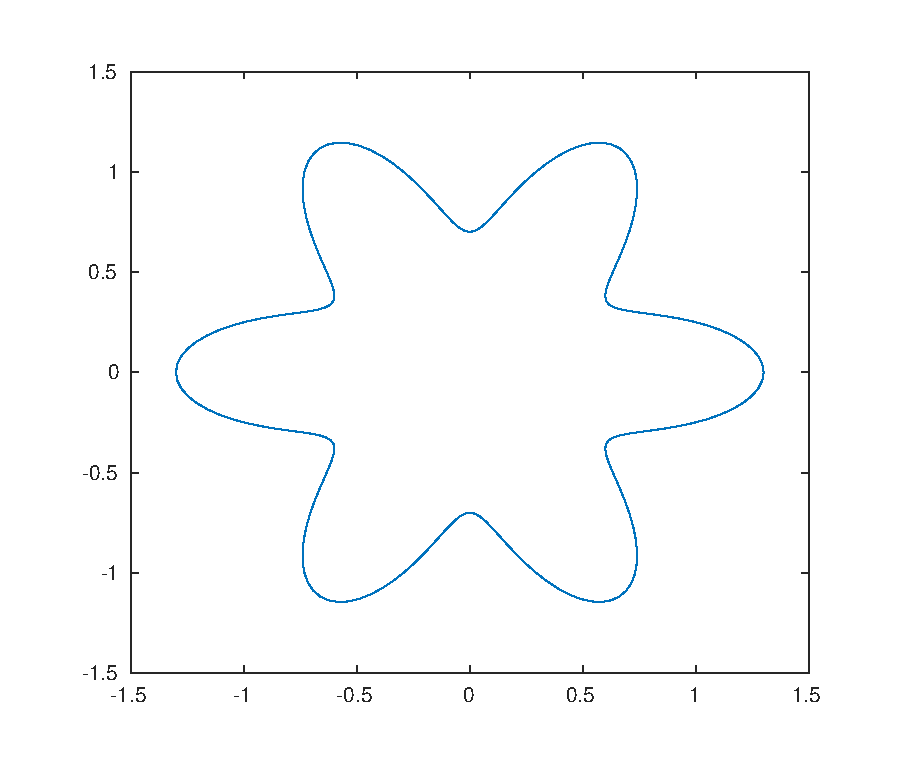
\includegraphics[width=7cm]{star.eps}                                           
  \caption{星型线}                        
\end{figure}

测试结果如表\ref{tab:starv1}和表\ref{tab:starv2}所示,所用误差范数
$\|\mathrm{E}\|_1$和$\|\mathrm{E}\|_{\infty}$是与参考解之间的网格1-范数
和无穷范数,参考解是对示踪点列进一步加密的结果。我们发现结果可以达到相应的收敛阶。

\begin{table}[htbp]
    \centering\begin{tabular}{c|ccccccc}
        \hline
         &$n=256$&ratio&512&ratio&1024&ratio&2048\\
        \hline
        $\|\mathrm{E}\|_1$&2.10e-1&1.99&5.29e-02&2.02&1.30e-2&2.07&3.11e-3\\
        \hline
        $\|\mathrm{E}\|_{\infty}$&1.02e+0&1.93&2.68e-1&2.00&6.71e-2&2.07&1.60e-2\\
        \hline
    \end{tabular}
    \caption{星型线测例: 误差及收敛阶,$r = 2$}
    \label{tab:starv1}
  \end{table}

  \begin{table}[htbp]
    \centering\begin{tabular}{c|ccccccc}
        \hline
         &$n=256$&ratio&512&ratio&1024&ratio&2048\\
        \hline
        $\|\mathrm{E}\|_1$&5.83e-2&3.78&4.24e-3&3.96&2.72e-4&4.00&1.70e-5\\
        \hline
        $\|\mathrm{E}\|_{\infty}$&3.27e-1&3.53&2.82e-2&3.89&1.91e-3&3.98&1.21e-4\\
        \hline
    \end{tabular}
    \caption{星型线测例: 误差及收敛阶,$r = 4$}
    \label{tab:starv2}
  \end{table}
  \newpage
\section{界面追踪测试}
下面将使用已经实现的二维MARS方法对曲率流进行界面追踪测试。使用的时间积
分方法为 ESDIRK ,分别对单位圆测例和星型线测例验证其精度。相应的
速度场测试已经说明了右端项的计算可以达到相应的精度。
\subsection{单位圆测例}

本测试模拟曲率流对单位圆的作用。初始曲线满足\eqref{eq:circle}式,
取终止时间$t_e=0.375$,此时曲线收缩成半径为 0.5 的圆。测试结果如表\ref{tab:circle1}和表\ref{tab:circle2}所示,所用误差范数$\|\mathrm{E}\|_1$是用计算出的三次样条曲线和用准确解正圆上的点生成的三次样条曲线求内部区域间近似异或面积得出的。我们发现结果可以达到相应的收敛阶。

\begin{table}[htbp]
    \centering\begin{tabular}{c|ccccccc}
        \hline
         $n$&64&ratio&128&ratio&256&ratio&512\\
                \hline
         $k$&1e-3&&5e-4&&2.5e-4&&1.25e-4\\
        \hline
        $\|\mathrm{E}\|_1$&7.52e-3&1.99&1.89e-3&2.00&4.73e-4&2.00&1.18e-4\\
        \hline
        CPU time(s)&2.54e+0&2.51&1.44e+1&2.72&9.50e+1&3.30&9.33e+2\\
        \hline
      \end{tabular}
    \caption{单位圆测例: 终止时间$t_e = 0.375$, $h_L=4\pi/n$,$r_{\text{tiny}}=0.1$,
      $\text{Order} = 2$}
    \label{tab:circle1}
  \end{table}

  \begin{table}[htbp]
    \centering\begin{tabular}{c|ccccc}
        \hline
         $n$&64&ratio&128&ratio&256\\
                \hline
         $k$&1e-3&&5e-4&&2.5e-4\\
        \hline
        $\|\mathrm{E}\|_1$&1.62e-6&4.00&1.01e-7&4.00&6.33e-9\\
        \hline
        CPU time(s)&1.26e+1&2.61&7.68e+1&3.11&6.62e+2\\
        \hline
      \end{tabular}
    \caption{单位圆测例: 终止时间$t_e = 0.375$, $h_L=4\pi/n$,$r_{\text{tiny}}=0.1$,
      $\text{Order} = 4$}
    \label{tab:circle2}
  \end{table}
  中间步的计算结果图如图\ref{fig:circlemidstep}所示。

\begin{figure}[H]
	\centering  %图片全局居中
	\subfigure[$t=0$]{
		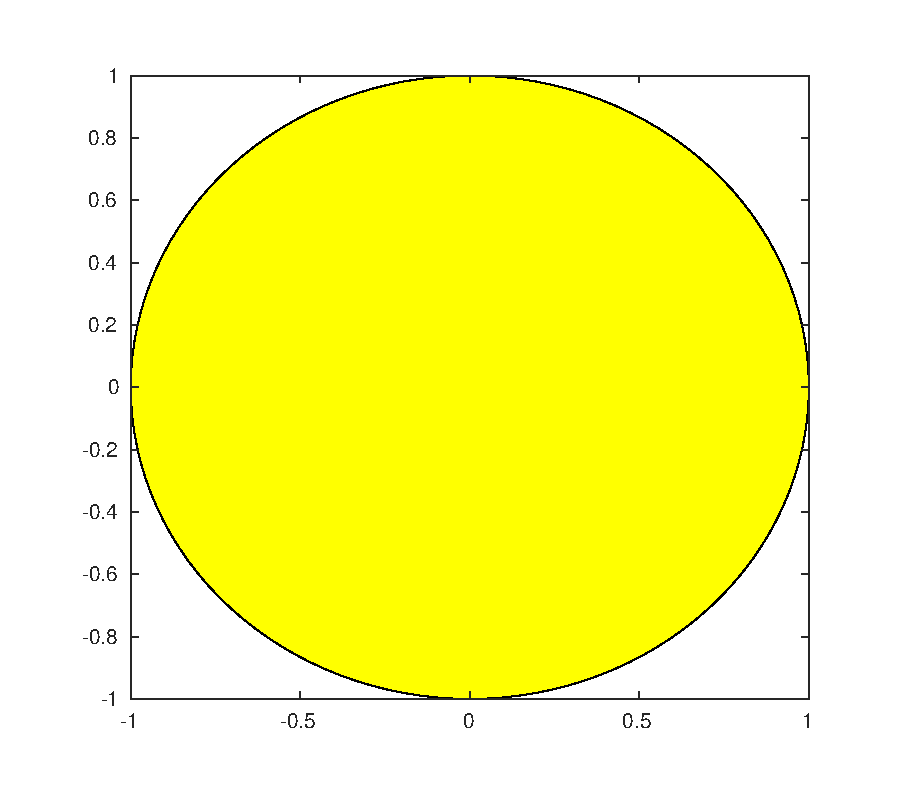
\includegraphics[width=0.4\linewidth]{circle_originfill.eps}
    }
    \subfigure[$t=0.125$]{
        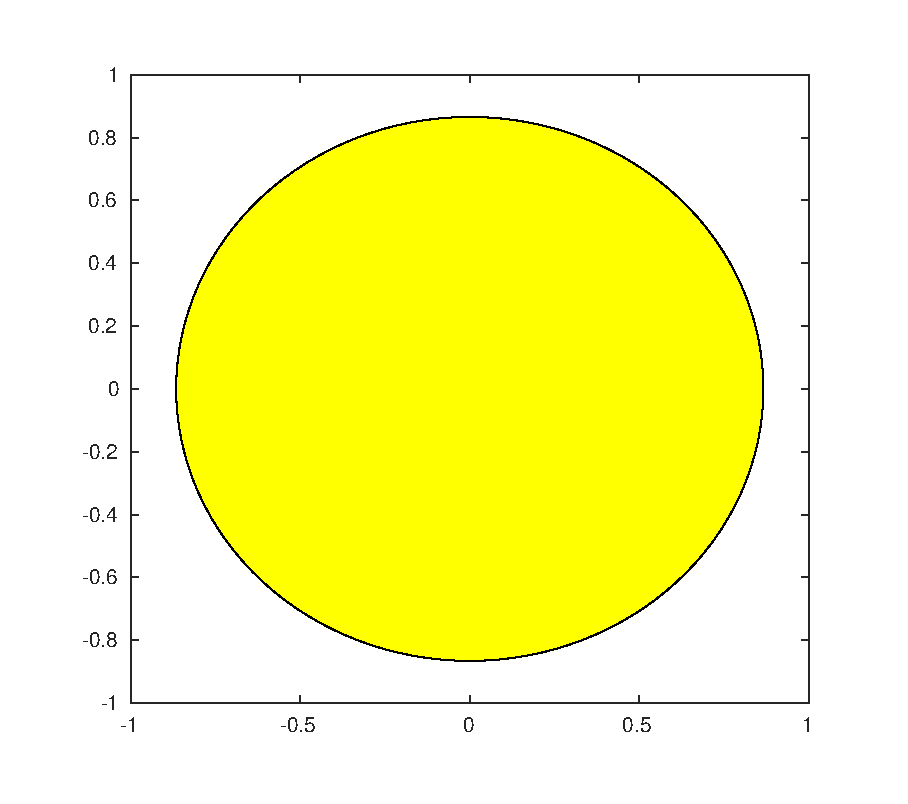
\includegraphics[width=0.4\linewidth]{circle_ESDIRK128_0.125.eps}
    }\\
    \subfigure[$t=0.25$]{
		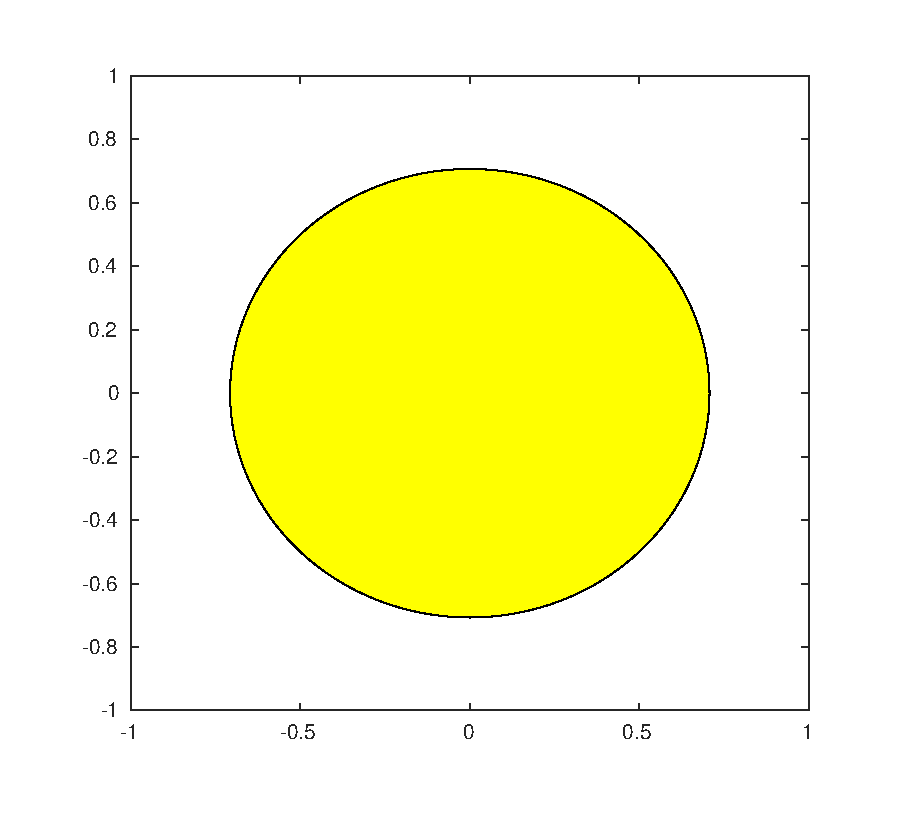
\includegraphics[width=0.4\linewidth]{circle_ESDIRK128_0.25.eps}
    }
    \subfigure[$t=0.375$]{
        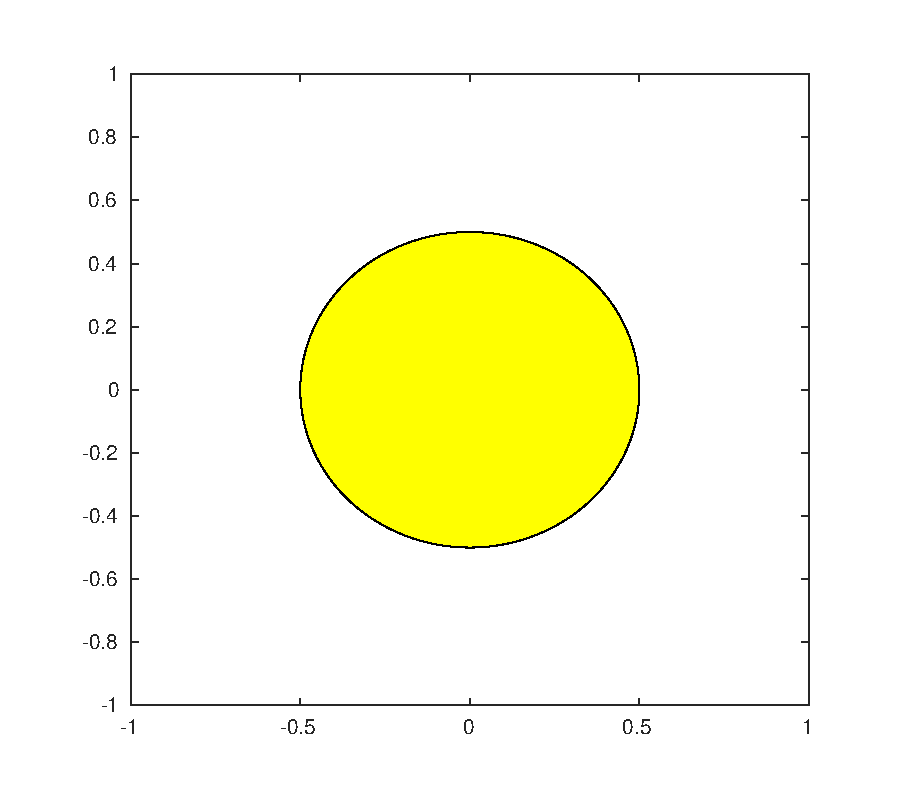
\includegraphics[width=0.4\linewidth]{circle_ESDIRK128_0.375.eps}
    }
    \caption{单位圆测例: 中间步计算结果图,所用参数为 $n=128$,$k=$ 5e-4,$r_\mathrm{tiny}=0.01$。}
    \label{fig:circlemidstep}
\end{figure}

  \subsection{星型线测例}

本测试模拟曲率流对星型曲线的作用。初始星型曲线由\eqref{eq:star}式给出,
取终止时间$t_e=0.4$,此时曲线收缩成半径为$\sqrt{49/200}$,圆心位于原点
的正圆。
\subsubsection{显式方法}
下面是用显式积分方法 ERK 的计算结果:
\begin{figure}[H]
	\centering  %图片全局居中
	\subfigure[$n=128$]{
		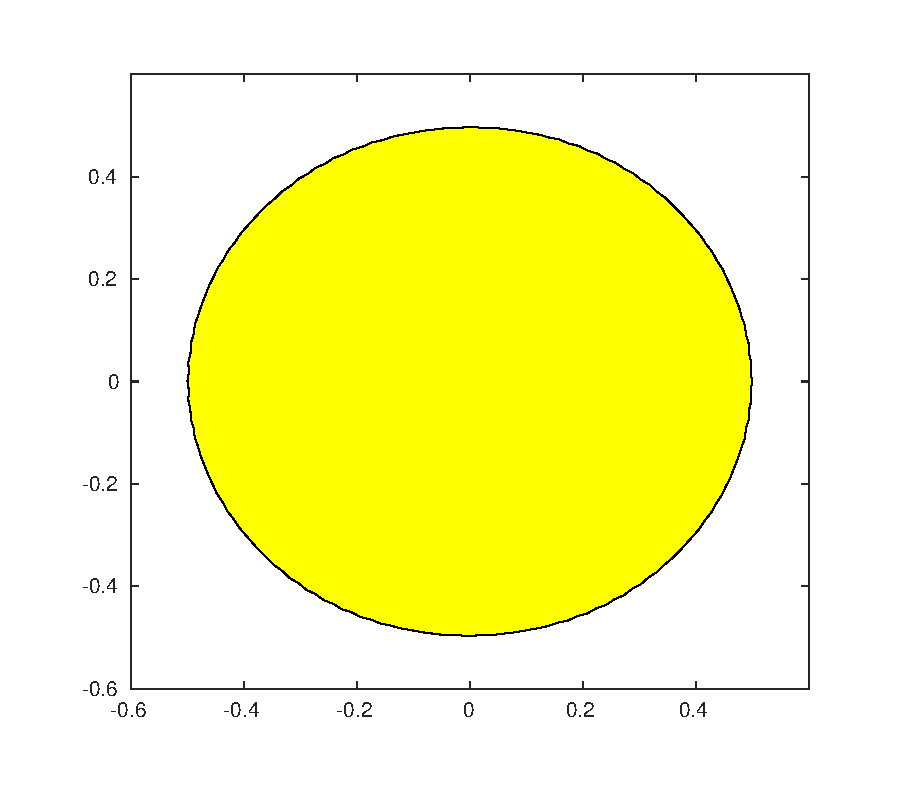
\includegraphics[width=0.3\linewidth]{star_ERK128_0.4.eps}
    }
	\subfigure[$n=256$]{
		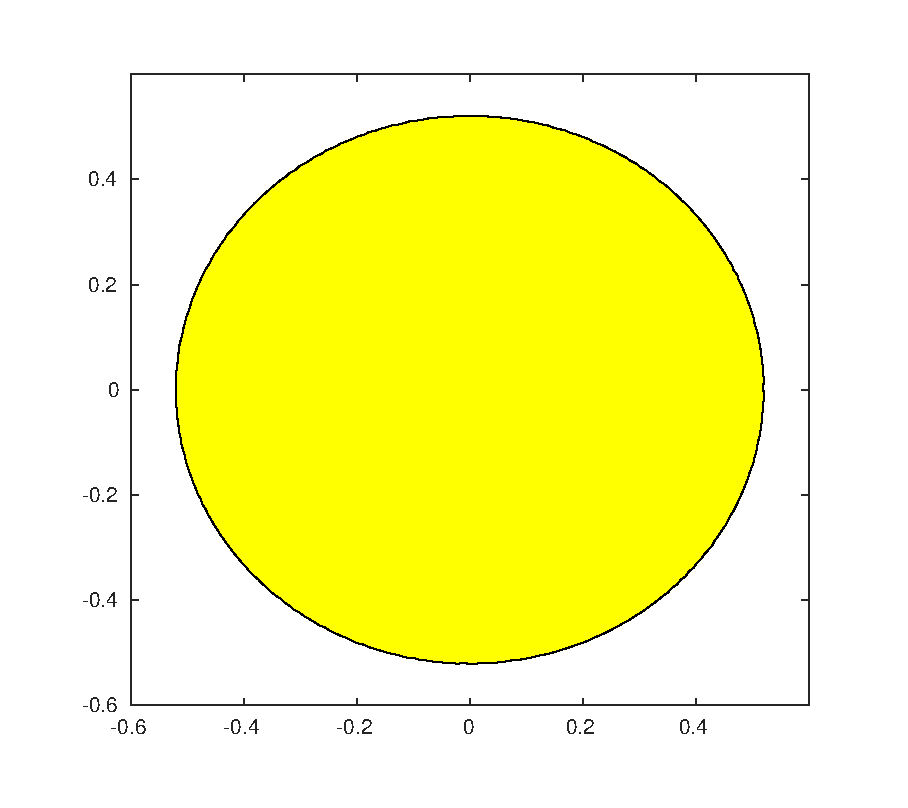
\includegraphics[width=0.3\linewidth]{star_ERK256_0.4.eps}
    }
    \subfigure[$n=512$]{
        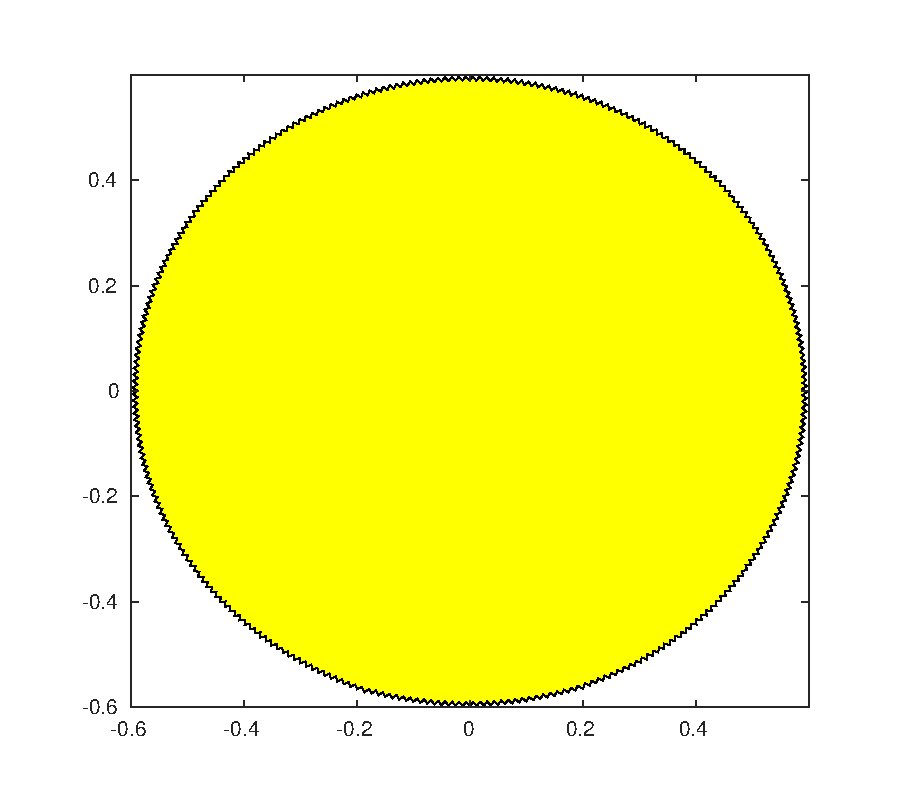
\includegraphics[width=0.3\linewidth]{star_ERK512_0.4.eps}
    }
    \caption{星型线测例: ERK,所用参数分别为 $n=128$,$k=$ 2e-4;
      $n=256$,$k=$ 1e-4和$n=512$,$k=$ 5e-5。终止时间$t_e = 0.4$,$h_L=4\pi/n$,$r_{\text{tiny}}=0.1$,
      $\text{Order} = 4$}
    \label{fig:star1}
\end{figure}
\begin{table}[htbp]
    \centering\begin{tabular}{c|ccc}
        \hline
         $n$&128&256&512\\
                \hline
         $k$&2e-4&1e-4&5e-5\\
        \hline
        $\|\mathrm{E}\|_1$&8.54e-3&7.89e-2&3.04e-1\\
        \hline
      \end{tabular}
    \caption{星型线测例: ERK,终止时间$t_e = 0.4$, $h_L=4\pi/n$,$r_{\text{tiny}}=0.1$,
      $\text{Order} = 4$}
    \label{tab:star1}
  \end{table}
  注意到当初始示踪点数$n$增大时,误差反而增大。这是因为显式积分方法在
  计算曲率流问题时是不稳定的。
\subsubsection{隐式方法}
下面使用四阶隐式积分方法 ESDIRK 进行测试。误差与CPU时间的测试结果如表\ref{tab:star2}所示,所用误差范数$\|\mathrm{E}\|_1$是用计算出的三次样条曲线和用准确解正圆上的点生成的三次样条曲线求内部区域间近似异或面积得出的。推测随着$n$增大,误差的收敛阶可以达到四阶精度。
\begin{table}[htbp]
    \centering\begin{tabular}{c|ccccc}
        \hline
         $n$&64&ratio&128&ratio&256\\
                \hline
         $k$&2e-4&&1e-4&&5e-5\\
        \hline
        $\|\mathrm{E}\|_1$&2.21e-3&2.38&4.23e-4&3.28&4.37e-5\\
        \hline
        CPU time(s)&8.82e+1&2.56&5.19e+2&3.19&7.73e+3\\
        \hline
      \end{tabular}
    \caption{星型线测例: ESDIRK,终止时间$t_e = 0.4$, $h_L=4\pi/n$,$r_{\text{tiny}}=0.1$,
      $\text{Order} = 4$}
    \label{tab:star2}
  \end{table}\\  
中间步的计算结果图如图\ref{fig:starmidstep}所示。
\newpage
\begin{figure}[H]
	\centering  %图片全局居中
	\subfigure[$t=0$]{
		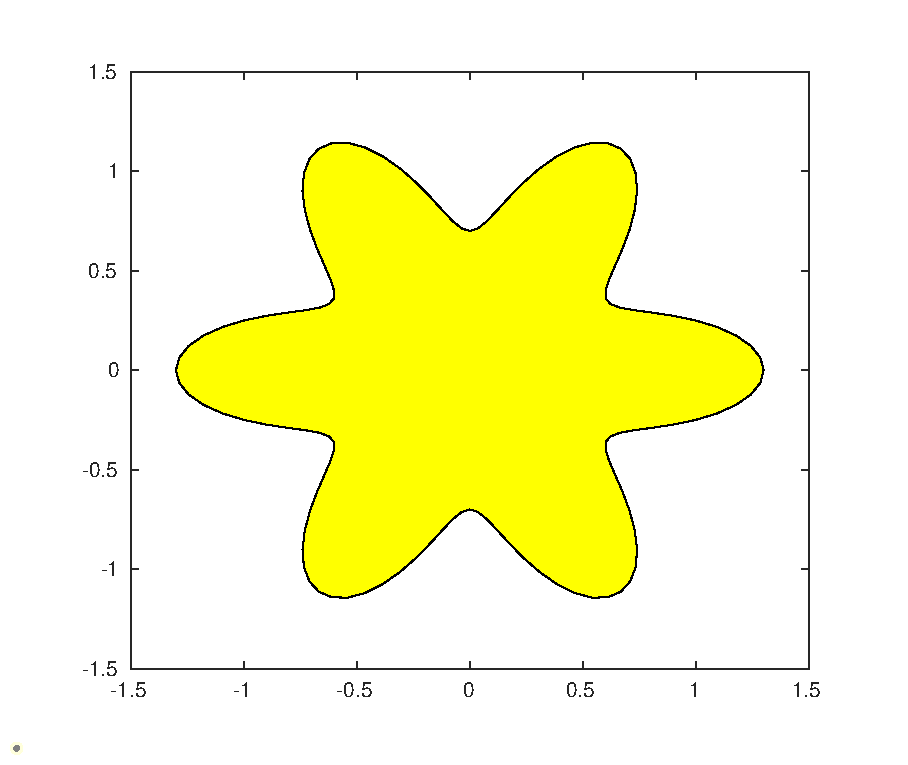
\includegraphics[width=0.3\linewidth]{star_originfill.eps}
    }
	\subfigure[$t=0.025$]{
		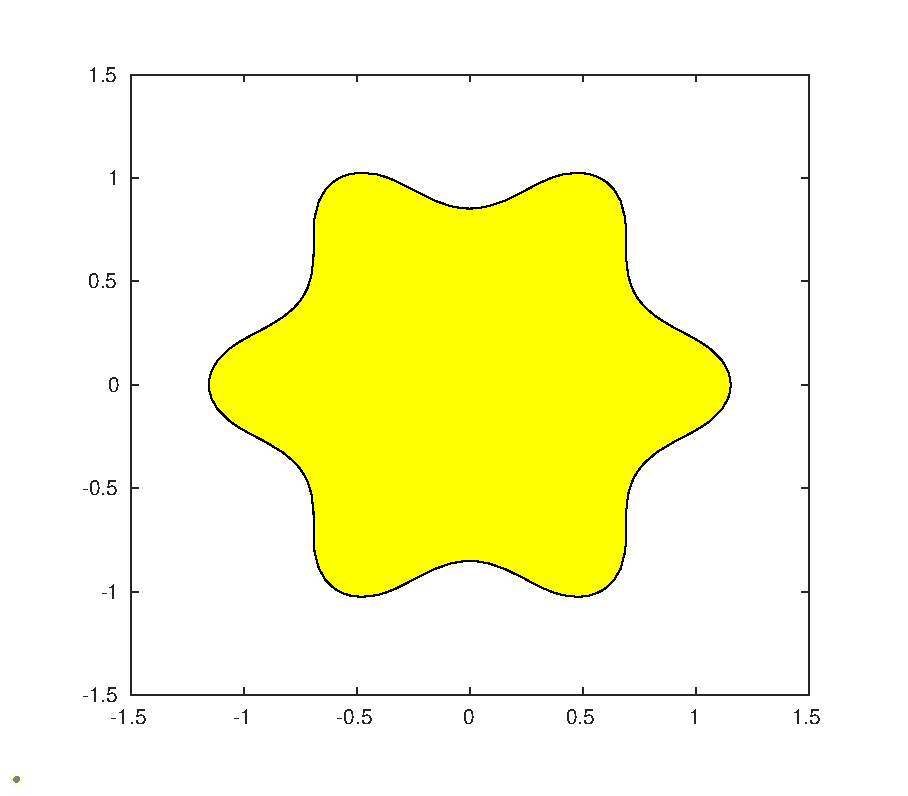
\includegraphics[width=0.3\linewidth]{star_ESDIRK128_0.025.eps}
    }
    \subfigure[$t=0.05$]{
        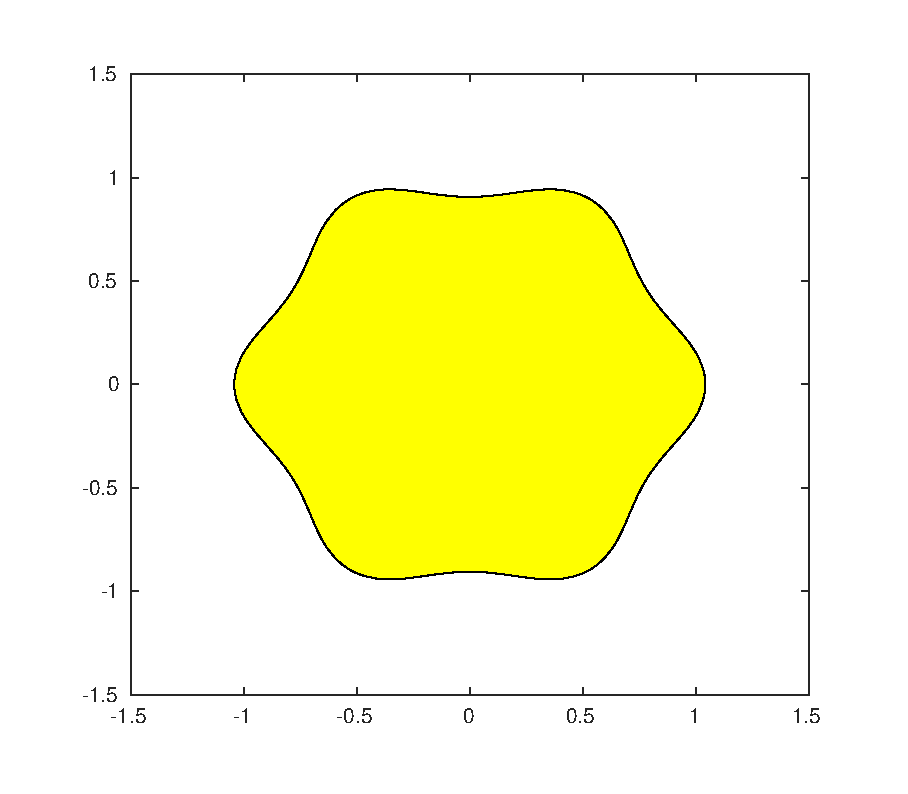
\includegraphics[width=0.3\linewidth]{star_ESDIRK128_0.05.eps}
    }\\
    \subfigure[$t=0.075$]{
		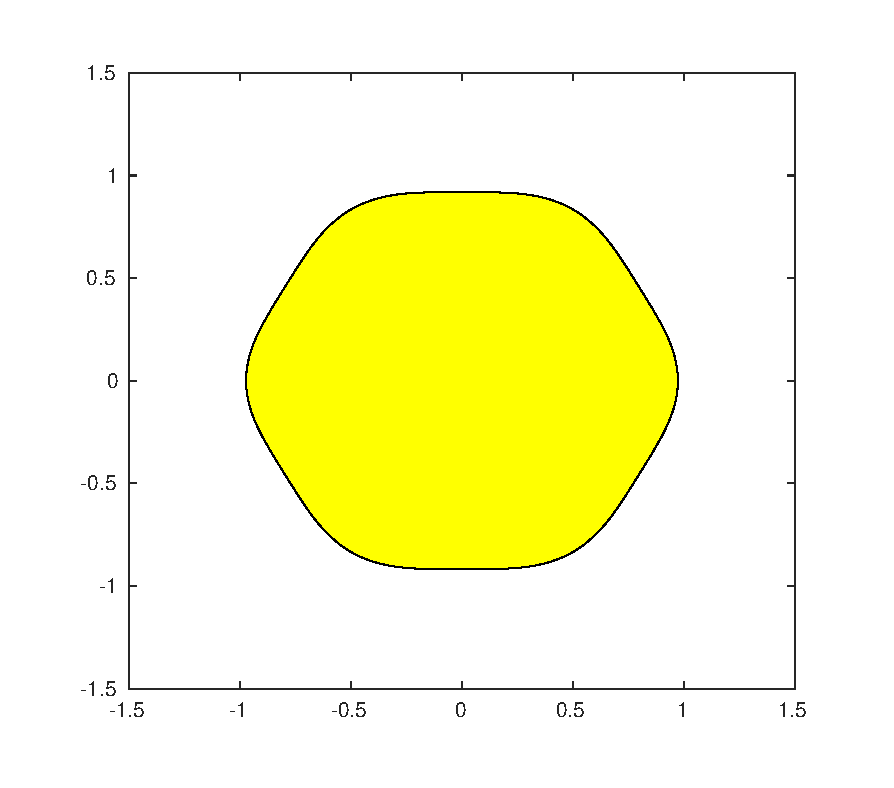
\includegraphics[width=0.3\linewidth]{star_ESDIRK128_0.075.eps}
    }
	\subfigure[$t=0.1$]{
		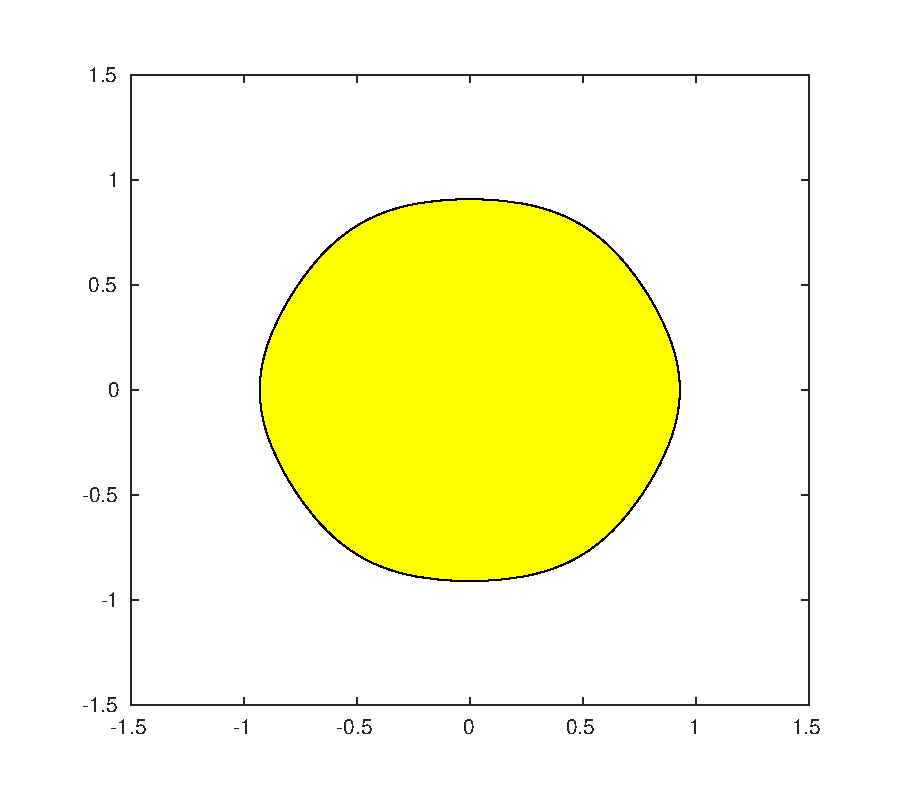
\includegraphics[width=0.3\linewidth]{star_ESDIRK128_0.1.eps}
    }
    \subfigure[$t=0.15$]{
        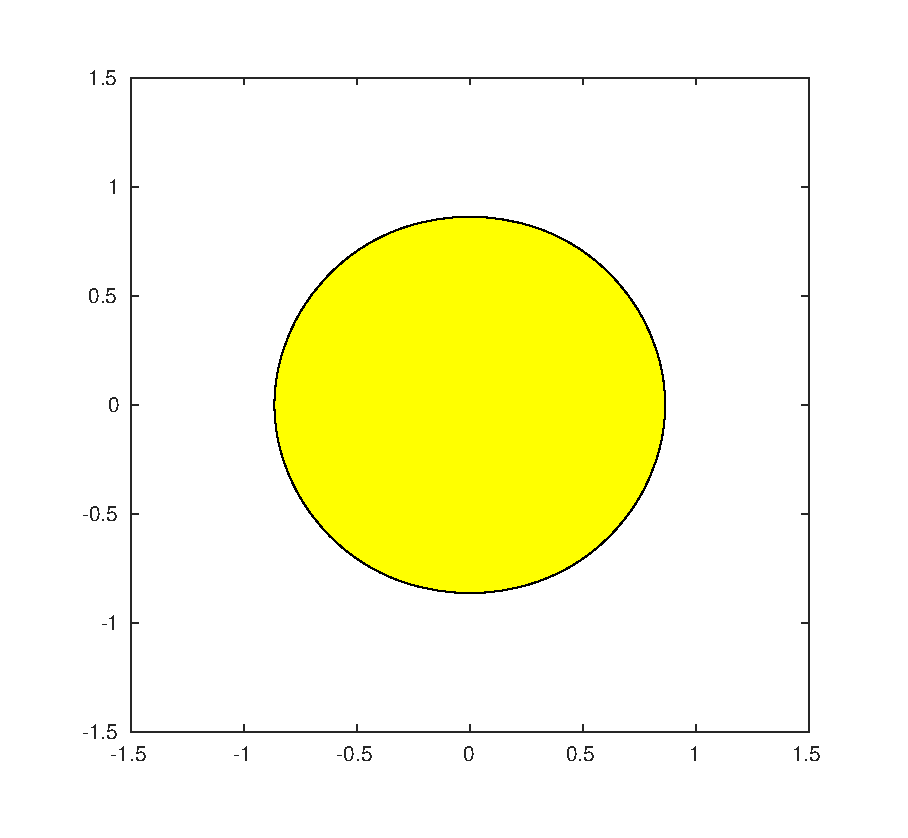
\includegraphics[width=0.3\linewidth]{star_ESDIRK128_0.15.eps}
    }\\
    \subfigure[$t=0.2$]{
		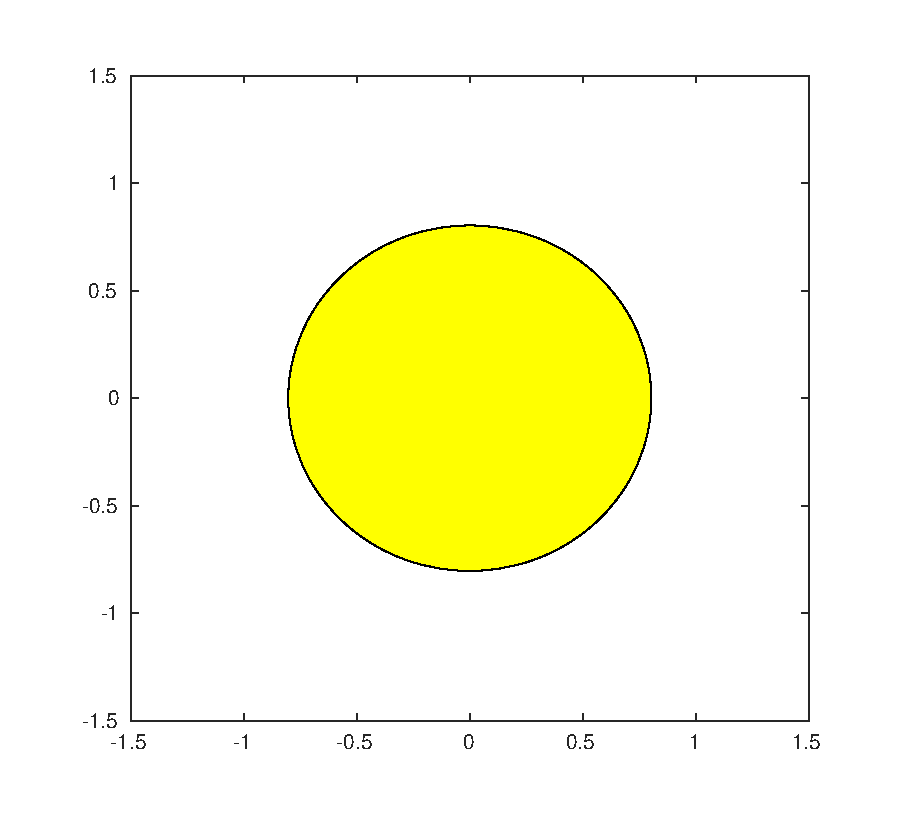
\includegraphics[width=0.3\linewidth]{star_ESDIRK128_0.2.eps}
    }
	\subfigure[$t=0.3$]{
		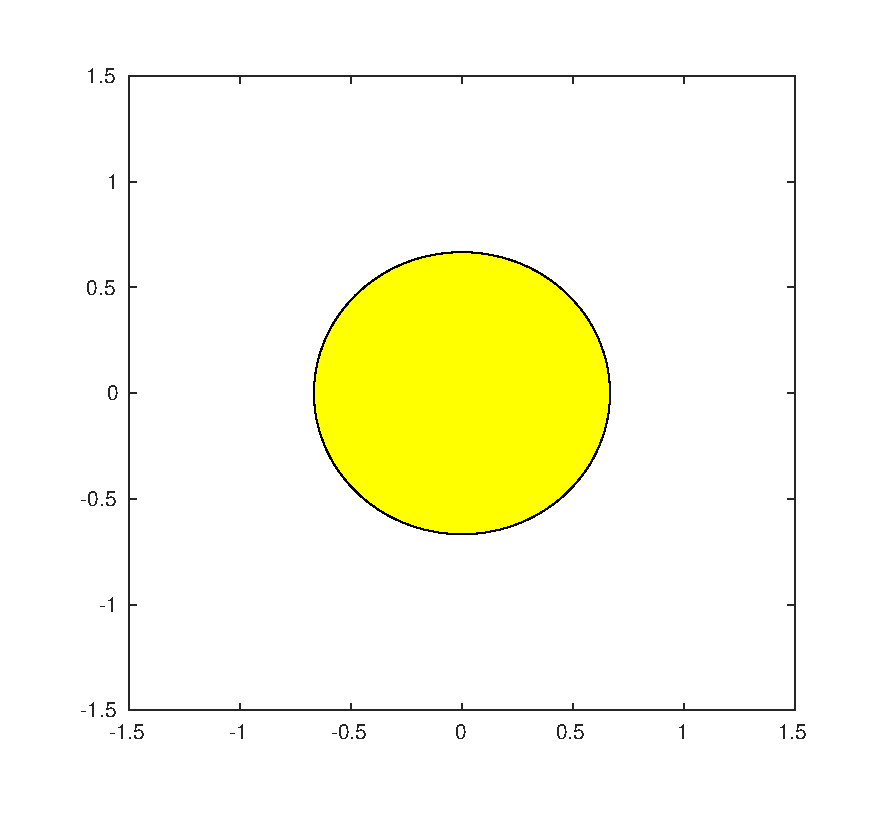
\includegraphics[width=0.3\linewidth]{star_ESDIRK128_0.3.eps}
    }
    \subfigure[$t=0.4$]{
        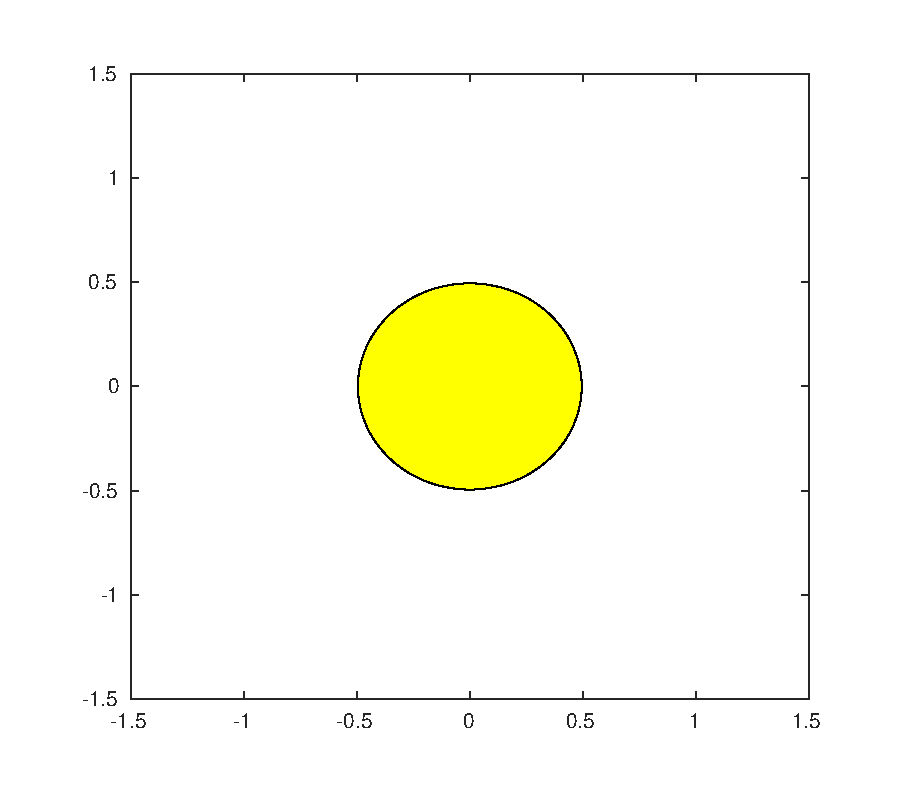
\includegraphics[width=0.3\linewidth]{star_ESDIRK128_0.4.eps}
    }
    \caption{星型线测例: 中间步计算结果图,所用参数为 $n=128$,$k=$ 1e-4,$r_\mathrm{tiny}=0.01$。}
    \label{fig:starmidstep}
\end{figure}



\end{document}
